\newcommand{\RingSegment}[6]{%
% #1 = center coordinate
% #2 = inner radius
% #3 = outer radius
% #4 = start angle
% #5 = delta angle
% #6 = TikZ style
\fill[#6]
  (#1) ++(#4:#2)
  arc[start angle=#4, delta angle=#5, radius=#2]
  -- ++(#4+#5:#3-#2)
  arc[start angle=#4+#5, delta angle=-#5, radius=#3]
  -- cycle;
}
\newcommand{\RingLabel}[5]{%
% #1 = center coordinate
% #2 = radius
% #3 = start angle
% #4 = delta angle
% #5 = text
  \pgfmathsetmacro{\angTmp}{#3 + 0.5*#4}
  \pgfmathsetmacro{\rotTmp}{\angTmp}
  \pgfmathsetmacro{\rotTmp}{%
      (\angTmp < 240) ? \angTmp + 180 : ((\angTmp < 300) ? \angTmp + 90 : \angTmp)
    }
  \node[
    font=\bfseries\tiny,
    align=center,
    rotate=\rotTmp
  ] at ($ (#1) + (\angTmp:#2) $) {#5};
}
\newcommand{\RingLabelCurved}[5]{%
% #1 = center
% #2 = radius
% #3 = start angle
% #4 = delta angle
% #5 = text
  \pgfmathsetmacro{\aMid}{#3 + 0.5*#4}
  \path[
    decorate,
    decoration={
      text along path,
      text={|\bfseries\scriptsize|#5},
      text align=center,
      raise=0.5ex
    }
  ]
  (#1) ++(#3:#2)
  arc[start angle=#3, delta angle=#4, radius=#2];
}
\newcommand{\InputOutputBox}[7]{%
    \node[align=justify, anchor=#1, text width=#3, minimum width=#3, minimum height=#2, fill=#4, rounded corners=2mm, font=\fontsize{1pt}{1pt}\selectfont] at (#5) 
          {%
              \textbf{Input:} #6\newline
              \textbf{Output:} #7
    };
}


\begin{figure*}[h!tb]
    \centering

    \begin{tikzpicture}        
        \node[anchor=center] (refMap) at (0,0) {};

        % radii: inner just outside image, outer controls thickness
        \def\rInner{0.4*\BenImgWidth}
        \def\rMid{0.85*\BenImgWidth}
        \def\rOuter{1.25*\BenImgWidth}
        \def\lineSep{1pt}
        \pgfmathsetmacro{\rLabelInner}{1.9}
        \pgfmathsetmacro{\rLabelMid}{2.1}
        \pgfmathsetmacro{\rLabelOuter}{2.5}
        
        \def\aStart{90}
        \def\aBin{136.6}
        \def\aBB{83.1}
        \def\aCap{17.5}
        \def\aMCQ{122.8}
        
        % inner segments
        \RingSegment{refMap}{\rInner}{\rMid}{\aStart}{\aBin}{Orchid!42.5, draw=white, line width=\lineSep}
        \RingSegment{refMap}{\rInner}{\rMid}{\aStart+\aBin}{\aBB}{red!37.5,draw=white,line width=\lineSep}
        \RingSegment{refMap}{\rInner}{\rOuter}{\aStart+\aBin+\aBB}{\aCap}{yellow!50,draw=white,line width=\lineSep}
        \RingSegment{refMap}{\rInner}{\rMid}{\aStart+\aBin+\aBB+\aCap}{\aMCQ}{YellowGreen!40,draw=white,line width=\lineSep}
        \RingLabelCurved{refMap}{\rLabelInner}{\aStart}{\aBin}{Binary VQA}
        \RingLabelCurved{refMap}{0.85*\rLabelInner}{\aStart+\aBin}{\aBB}{Ref. Exp.}
        \RingLabelCurved{refMap}{\rLabelInner}{\aStart+\aBin}{\aBB}{Detection}
        \RingLabel{refMap}{\rLabelMid}{\aStart+\aBin+\aBB}{\aCap}{Captioning}
        \RingLabelCurved{refMap}{\rLabelInner}{\aStart+\aBin+\aBB+\aCap}{\aMCQ}{Multiple-Choice VQA}

        \def\bBinAdj{31.8}
        \def\bBinArea{34.9}
        \def\bBinCount{34.9}
        \def\bBinPresence{34.9}
        \RingSegment{refMap}{\rMid}{\rOuter}{\aStart}{\bBinAdj}{Orchid!15, draw=white, line width=\lineSep}
        \RingSegment{refMap}{\rMid}{\rOuter}{\aStart+\bBinAdj}{\bBinArea}{Orchid!30, draw=white, line width=\lineSep}
        \RingSegment{refMap}{\rMid}{\rOuter}{\aStart+\bBinAdj+\bBinArea}{\bBinCount}{Orchid!45, draw=white, line width=\lineSep}
        \RingSegment{refMap}{\rMid}{\rOuter}{\aStart+\bBinAdj+\bBinArea+\bBinCount}{\bBinPresence}{Orchid!60, draw=white, line width=\lineSep}
        \RingLabel{refMap}{\rLabelOuter}{\aStart}{\bBinAdj}{\adjacencyABBR}
        \RingLabel{refMap}{\rLabelOuter}{\aStart+\bBinAdj}{\bBinArea}{\areaABBR}
        \RingLabel{refMap}{\rLabelOuter}{\aStart+\bBinAdj+\bBinArea}{\bBinCount}{\countABBR}
        \RingLabel{refMap}{\rLabelOuter}{\aStart+\bBinAdj+\bBinArea+\bBinCount}{\bBinPresence}{\presenceABBR}
        
        \def\bBBPoint{43.1}
        \def\bBBRef{40.0}
        \RingSegment{refMap}{\rMid}{\rOuter}{\aStart+\aBin}{\bBBPoint}{red!25,draw=white,line width=\lineSep}
        \RingSegment{refMap}{\rMid}{\rOuter}{\aStart+\aBin+\bBBPoint}{\bBBRef}{red!50,draw=white,line width=\lineSep}
        \RingLabel{refMap}{\rLabelOuter}{\aStart+\aBin}{\bBBPoint}{Ref. Point\\Detection}
        \RingLabel{refMap}{\rLabelOuter}{\aStart+\aBin+\bBBPoint}{\bBBRef}{Ref. LULC\\Detection}
        
        \def\bCap{17.5}
        
        \def\bMCQAdj{14.3}
        \def\bMCQArea{17.5}
        \def\bMCQClimate{17.5}
        \def\bMCQCount{17.5}
        \def\bMCQCountry{17.5}
        \def\bMCQPresence{17.5}
        \def\bMCQRelPos{3.7}
        \def\bMCQSeason{17.5}
        \RingSegment{refMap}{\rMid}{\rOuter}{\aStart+\aBin+\aBB+\aCap}{\bMCQAdj}{YellowGreen!10,draw=white,line width=\lineSep}
        \RingSegment{refMap}{\rMid}{\rOuter}{\aStart+\aBin+\aBB+\aCap+\bMCQAdj}{\bMCQArea}{YellowGreen!20,draw=white,line width=\lineSep}
        \RingSegment{refMap}{\rMid}{\rOuter}{\aStart+\aBin+\aBB+\aCap+\bMCQAdj+\bMCQArea}{\bMCQClimate}{YellowGreen!30,draw=white,line width=\lineSep}
        \RingSegment{refMap}{\rMid}{\rOuter}{\aStart+\aBin+\aBB+\aCap+\bMCQAdj+\bMCQArea+\bMCQClimate}{\bMCQCount}{YellowGreen!40,draw=white,line width=\lineSep}
        \RingSegment{refMap}{\rMid}{\rOuter}{\aStart+\aBin+\aBB+\aCap+\bMCQAdj+\bMCQArea+\bMCQClimate+\bMCQCount}{\bMCQCountry}{YellowGreen!50,draw=white,line width=\lineSep}
        \RingSegment{refMap}{\rMid}{\rOuter}{\aStart+\aBin+\aBB+\aCap+\bMCQAdj+\bMCQArea+\bMCQClimate+\bMCQCount+\bMCQCountry}{\bMCQPresence}{YellowGreen!60,draw=white,line width=\lineSep}
        \RingSegment{refMap}{\rMid}{\rOuter}{\aStart+\aBin+\aBB+\aCap+\bMCQAdj+\bMCQArea+\bMCQClimate+\bMCQCount+\bMCQCountry+\bMCQPresence}{\bMCQRelPos}{YellowGreen!70,draw=white,line width=\lineSep}
        \RingSegment{refMap}{\rMid}{\rOuter}{\aStart+\aBin+\aBB+\aCap+\bMCQAdj+\bMCQArea+\bMCQClimate+\bMCQCount+\bMCQCountry+\bMCQPresence+\bMCQRelPos}{\bMCQSeason}{YellowGreen!80,draw=white,line width=\lineSep}
        \RingLabel{refMap}{\rLabelOuter}{\aStart+\aBin+\aBB+\aCap}{\bMCQAdj}{\adjacencyABBR}
        \RingLabel{refMap}{\rLabelOuter}{\aStart+\aBin+\aBB+\aCap+\bMCQAdj}{\bMCQArea}{\areaABBR}
        \RingLabel{refMap}{\rLabelOuter}{\aStart+\aBin+\aBB+\aCap+\bMCQAdj+\bMCQArea}{\bMCQClimate}{\climateABBR}
        \RingLabel{refMap}{\rLabelOuter}{\aStart+\aBin+\aBB+\aCap+\bMCQAdj+\bMCQArea+\bMCQClimate}{\bMCQCount}{\countABBR}
        \RingLabel{refMap}{\rLabelOuter}{\aStart+\aBin+\aBB+\aCap+\bMCQAdj+\bMCQArea+\bMCQClimate+\bMCQCount}{\bMCQCountry}{\countryABBR}
        \RingLabel{refMap}{\rLabelOuter}{\aStart+\aBin+\aBB+\aCap+\bMCQAdj+\bMCQArea+\bMCQClimate+\bMCQCount+\bMCQCountry}{\bMCQPresence}{\presenceABBR}
        \RingLabel{refMap}{\rLabelOuter}{\aStart+\aBin+\aBB+\aCap+\bMCQAdj+\bMCQArea+\bMCQClimate+\bMCQCount+\bMCQCountry+\bMCQPresence}{\bMCQRelPos}{\relativepositionABBR}
        \RingLabel{refMap}{\rLabelOuter}{\aStart+\aBin+\aBB+\aCap+\bMCQAdj+\bMCQArea+\bMCQClimate+\bMCQCount+\bMCQCountry+\bMCQPresence+\bMCQRelPos}{\bMCQSeason}{\seasonABBR}

        \begin{scope}
          \clip[rounded corners=5mm]
            ($(refMap)+(-0.5*\BenImgWidth,-0.5*\BenImgWidth)$)
            rectangle
            ($(refMap)+( 0.5*\BenImgWidth, 0.5*\BenImgWidth)$);
        
          \node[anchor=center, inner sep=0pt] at (refMap)
            %{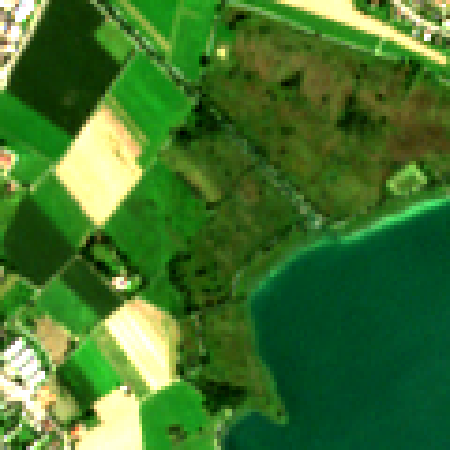
\includegraphics[width=\BenImgWidth]{figures/dataset/samples/_tci_S2A_MSIL2A_20170818T103021_N9999_R108_T32TMT_61_44.png}};
            {\begin{tikzpicture}[scale=0.9]
  % outer disk
  \fill[BlueGreen!20] (0,0) circle (1.2);
  \draw[white, line width=1pt] (0,0) circle (1.2);
  \draw[BlueGreen!50, line width=0.6pt] (0,0) circle (1);

  % latitude / longitude hints
  \draw[BlueGreen!60, line width=0.6pt] (-1.0,0) arc (180:360:1.0 and 0.35);
  \draw[BlueGreen!40, line width=0.3pt, dashed] (-1.0,0) arc (180:0:1.0 and 0.35);
  
  
  \draw[BlueGreen!40, line width=0.3pt, dashed] (0,-1.0) arc (-90:90:0.35 and 1.0);
  \draw[BlueGreen!60, line width=0.6pt] (0,-1.0) arc (-90:-270:0.35 and 1.0);

  
  \draw[BlueGreen!50, line width=0.6pt] (0,0) circle (1);


  % text bars (.txt)
  \node at (-0.6, 0) {
\includegraphics[scale=0.021,decodearray={0 0.65 0 0.65 0 0.65}]{figures/ben_txt_logos/rsim_logo_weiss.png}};
  \fill[gray!70] (-0.2,-0.2) rectangle (0.8,-0.12);
  \fill[gray!70] (-0.2,-0.05) rectangle (0.65,0.03);
  \fill[gray!70] (-0.2,0.10) rectangle (0.75,0.18);

  % name
  %\node[font=\bfseries\scriptsize] at (0,-0.55) {BigEarthNet};
  \path[decorate,decoration={text along path,text={|\bfseries\notsotiny|BigEarthNet},text align=center,raise=-1.6ex}] (-1.0,0) arc (180:360:1.0 and 0.35);
  \node[font=\bfseries\small] at (0,-0.8) {\texttt{.txt}};
\end{tikzpicture}};
        \end{scope}
        
        \def\boxHeight{18mm}
        \def\boxWidth{20mm}  % 20mm
        \InputOutputBox{south east}{0.7*\boxHeight}{\boxWidth}{YellowGreen!60}{$(-\rOuter, -\rOuter) + (-.1,0)$}{Which season is shown in the satellite image? a)~Spring, b)~Summer, c)~Winter, d)~Autumn}{b}
        \InputOutputBox{north east}{0.7*\boxHeight}{\boxWidth}{Orchid!60}{$(-\rOuter, 0) + (-.1,-.05)$}{Are there regions of coastal wetlands in the satellite image?}{No}
        \InputOutputBox{south east}{0.7*\boxHeight}{\boxWidth}{Orchid!15}{$(-\rOuter, 0) + (-.1,.05)$}{Does any inland water border inland wetlands in this scene?}{Yes}
        \InputOutputBox{north east}{0.86*\boxHeight}{\boxWidth}{YellowGreen!40}{$(-\rOuter, \rOuter) + (-.1,0)$}{How many areas covered by urban fabric can be seen? a)~More than five, b)~3, c)~1, d)~0}{b}
        
        \InputOutputBox{south west}{\boxHeight}{\boxWidth}{red!25}{$(\rOuter, -\rOuter) + (.1,-.1)$}{Output a bounding box enclosing the land cover class instance positioned at <point>(0.83, 0.06)</point>.}{[0.49 0.0, 1.0 0.2]}
        \InputOutputBox{west}{\boxHeight}{\boxWidth}{red!50}{$(\rOuter, 0) + (.1,-.05)$}{Where can the <ref>largest area of urban fabric</ref> be found?}{[0.0 0.55, 0.2 1.0]}
        \InputOutputBox{north west}{\boxHeight}{\boxWidth}{YellowGreen!70}{$(\rOuter, \rOuter) + (.1,0)$}{What is the relative position of the arable land to the inland waters? a) to the left, b) to the bottom, c) to the top-right, d) to the top}{a}

        %\InputOutputBox{south}{\BenImgWidth}{64mm+2*\boxWidth-2*25mm}{yellow!50}{$(0, \rOuter) + (0,.1)$}{Describe the content of the image, including the region, climate zone, and land cover distribution.}{This satellite image, captured during the summer season in Switzerland, showcases a diverse landscape within the "temperate, no dry season, warm summer" climate zone. The dominant features are arable land (~526,000 sqm) and inland wetlands (~460,000 sqm), which are adjacent to each other. The arable land borders both inland wetlands and urban fabric (~149,000 sqm). Moreover, the inland wetlands are adjacent to both inland waters (~305,000 sqm) and urban fabric. Notably, the urban fabric is distributed over three individual marginal areas. The varied landscape presents a mix of agricultural areas, wetlands, water bodies, and artificial surfaces.}
        \InputOutputBox{south}{\BenImgWidth}{64mm+2*\boxWidth-2*24mm}{yellow!50}{$(0, \rOuter) + (0,.1)$}{Describe the content of the image, including the region, climate zone, and land cover distribution.}{This satellite image, captured during the summer season in Switzerland, showcases a diverse landscape within the "temperate, no dry season, warm summer" climate zone. The dominant features are arable land ($\sim$526,000 sqm) [...] are adjacent to both inland waters ($\sim$305,000 sqm) and urban fabric. Notably, the urban fabric is distributed over three individual marginal areas. The varied landscape presents a mix of agricultural areas, wetlands, water bodies, and artificial surfaces.}

        \begin{scope}
          % \clip[rounded corners=5mm]
          %   ($(-\rOuter, \rOuter) + (0,.1)$)
          %   rectangle
          %   ($(-\rOuter, \rOuter)+(-\BenImgWidth, \BenImgWidth) + (0,.1)$);
        
          \node[anchor=south east, inner sep=0pt] at ($(-\rOuter, \rOuter) + (0,.1)$)
            {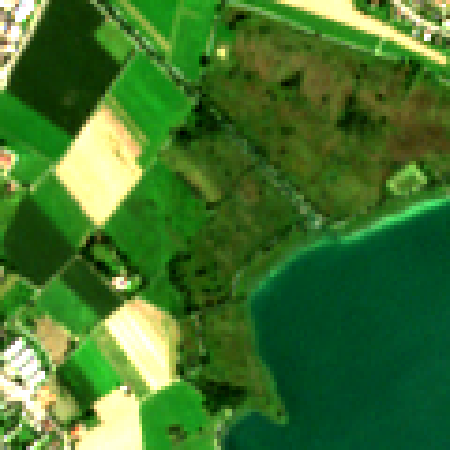
\includegraphics[width=\BenImgWidth]{figures/dataset/samples/_tci_S2A_MSIL2A_20170818T103021_N9999_R108_T32TMT_61_44.png}};
        \end{scope}
        \begin{scope}
          % \clip[rounded corners=5mm]
          %   ($(\rOuter, \rOuter) + (0,.1)$)
          %   rectangle
          %   ($(\rOuter, \rOuter)+(\BenImgWidth, \BenImgWidth) + (0,.1)$);
        
          \node[anchor=south west, inner sep=0pt] at ($(\rOuter, \rOuter) + (0,.1)$)
            {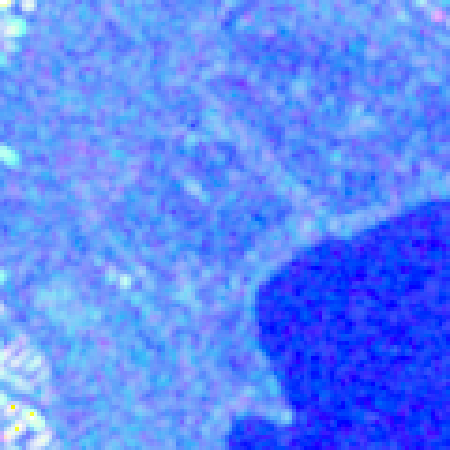
\includegraphics[width=\BenImgWidth]{figures/dataset/samples/_rtc_S2A_MSIL2A_20170818T103021_N9999_R108_T32TMT_61_44.png}};
        \end{scope}
    \end{tikzpicture} 

    \caption{\bentxt{} comprises \num{464 044} co-registered \ac{S1} and \ac{S2} images with diverse text annotations, resulting in a total of $\sim~\num{9.6}$ million \ac{S1}-\ac{S2}-text triplets. The dataset supports 15 tasks (Presence, Area, Counting, Adjacency, Relative Position, Country, Season, and Climate Zone, denoted as \presenceABBR, \areaABBR, \countABBR, \adjacencyABBR, \relativepositionABBR, \countryABBR, \seasonABBR, and \climateABBR, respectively) across 4 broad categories.}
    \label{fig:dataset_overview}
\end{figure*}